%%% Copyright (C) 2017 Vincent Goulet
%%%
%%% This file and all files included or input by this one (and
%%% recursively) are part of the project "The Best of Both Worlds:
%%% Using Blended Learning in Actuarial Science Courses - Actuarial
%%% Teaching Conference 2017"
%%% http://github.com/vigou3/ATC2017-blended-learning
%%%
%%% This work is licensed under a Creative Commons
%%% Attribution-ShareAlike 4.0 International License.
%%% http://creativecommons.org/licenses/by-sa/4.0/

\documentclass[aspectratio=1610,10pt,xcolor=x11names]{beamer}
  \usepackage{fontawesome}
  \usepackage{changepage}                % page licence
  \usepackage{tabularx}                  % page licence
  \usepackage{framed}                    % env. leftbar
  \usepackage[export]{adjustbox}         % cadre autour image
  \usepackage[overlay,absolute]{textpos} % covers
  \usepackage{metalogo}                  % logo \XeLaTeX

  %% ==================
  %%  Publication info
  %% ==================
  \renewcommand{\year}{2017}

  %% ===============================
  %%  Look and feel of the document
  %% ===============================

  %% Beamer theme
  \usetheme{metropolis}

  %% Additionnal colors
  \definecolor{link}{rgb}{0,0.4,0.6}        % internal links
  \definecolor{url}{rgb}{0.6,0,0}           % external links
  \definecolor{rouge}{rgb}{0.85,0,0.07}     % UL red stripe
  \definecolor{or}{rgb}{1,0.8,0}            % UL yellow stripe

  %% Hyperlinks
  \hypersetup{%
    pdfauthor = {Vincent Goulet},
    pdftitle = {The Best of Both Worlds: Using Blended Learning in Actuarial Science Courses},
    colorlinks = {true},
    linktocpage = {true},
    allcolors = {link},
    urlcolor = {url},
    pdfpagemode = {UseOutlines},
    pdfstartview = {Fit},
    bookmarksopen = {true},
    bookmarksnumbered = {true},
    bookmarksdepth = {subsection}}

  %% Bibliographie
  \bibliographystyle{francais}

  %% =====================
  %%  Nouvelles commandes
  %% =====================

  \newcommand{\link}[2]{\href{#1}{#2~\raisebox{-0.2ex}{\faExternalLink}}}
  \newcommand{\meta}[1]{\ensuremath\langle{\normalfont\itshape #1\/}\ensuremath\rangle}

  %% Link to GitHub on copyright page
  \newcommand{\viewsource}[1]{%
    \href{#1}{%
      \makebox[2.5mm]{\raisebox{-1pt}{\footnotesize\faGithub}}\;%
      {\sffamily View on GitHub}}}

  %%% =======
  %%%  Varia
  %%% =======

  %% Lengths used to compose front and rear covers.
  \newlength{\banderougewidth} \newlength{\banderougeheight}
  \newlength{\bandeorwidth}    \newlength{\bandeorheight}
  \newlength{\imageheight}     \newlength{\imagewidth}
  \newlength{\logoheight}
  \newlength{\gapwidth}

%  \includeonly{couverture-avant}

\begin{document}

%% frontmatter
\begingroup

\TPGrid{3}{36}
\textblockorigin{0mm}{0mm}
\setlength{\parindent}{0mm}
\setlength{\banderougewidth}{2\TPHorizModule}
\setlength{\banderougeheight}{\TPVertModule}
\setlength{\bandeorwidth}{\TPHorizModule}
\setlength{\bandeorheight}{\banderougeheight}
\setlength{\imageheight}{29\TPVertModule}
\setlength{\imagewidth}{3\TPHorizModule}
\setlength{\logoheight}{2.5\TPVertModule}
\setlength{\gapwidth}{0.75pt}
\addtolength{\bandeorwidth}{-\gapwidth}
\addtolength{\imageheight}{-\gapwidth}

\begin{frame}[plain]
  %% UL banner
  \begin{textblock*}{3\TPHorizModule}[0,1](0mm,30\TPVertModule)
    \textcolor{rouge}{\rule{\banderougewidth}{\banderougeheight}}% % red stripe
    \rule{\gapwidth}{0pt}%                                         % gap
    \textcolor{or}{\rule{\bandeorwidth}{\bandeorheight}}           % gold stripe
  \end{textblock*}

  %% UL logo
  \begin{textblock*}{\TPHorizModule}(2\TPHorizModule,31\TPVertModule)
    \rule{\gapwidth}{0pt}%                                     % gap
    \includegraphics[height=\logoheight,keepaspectratio=true]{ul_p}
  \end{textblock*}

  %% background image
  \begin{textblock*}{3\TPHorizModule}(0mm,0mm)
    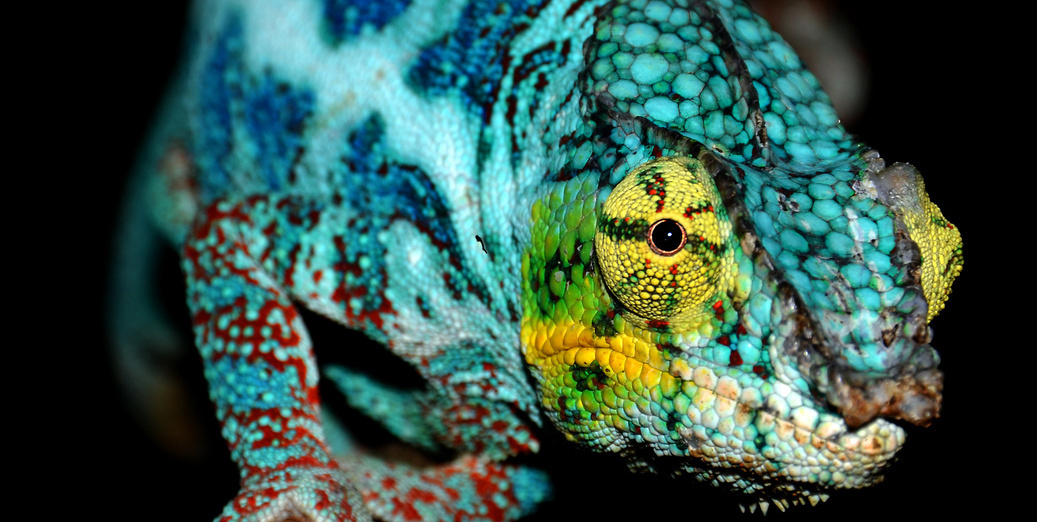
\includegraphics[height=\imageheight,width=\imagewidth]{furcifer-pardalis-nosy-faly}
  \end{textblock*}

  %% title
  \begin{textblock*}{2\TPHorizModule}(0.205\TPHorizModule,3.1\TPVertModule)
    %% Poor Man's (but simple!) shadow effect behind letters; needed
    %% to let the title stand out on the dark background
    \raggedright%
    \bfseries
    \fontsize{20}{20}\selectfont
    \textcolor{black}{%
      The Best of Both Worlds: \\
      Using Blended Learning \\
      in Actuarial Science Courses} \\
    \mdseries
    \fontsize{14}{18}\selectfont
    \textcolor{black}{Actuarial Teaching Conference 2017}
  \end{textblock*}
  \begin{textblock*}{2\TPHorizModule}(0.2\TPHorizModule,3\TPVertModule)
    \raggedright%
    \bfseries
    \fontsize{20}{20}\selectfont
    \textcolor{white}{%
      The Best of Both Worlds: \\
      Using Blended Learning \\
      in Actuarial Science Courses} \\
    \mdseries
    \fontsize{14}{18}\selectfont
    \textcolor{white}{Actuarial Teaching Conference 2017}
  \end{textblock*}

  %% date
  \begin{textblock*}{2\TPHorizModule}(0.2\TPHorizModule,26\TPVertModule)
    \fontsize{10}{12}\selectfont
    \textcolor{white}{June 27, 2017}
  \end{textblock*}
\end{frame}
\endgroup

%%% Local Variables:
%%% mode: latex
%%% TeX-engine: xetex
%%% TeX-master: "ATC2017-blended-learning"
%%% End:

\begingroup

\TPGrid{3}{36}
\textblockorigin{0mm}{0mm}
\begin{frame}[plain]
  %% title
  \begin{textblock*}{2\TPHorizModule}(0.2\TPHorizModule,3\TPVertModule)
    \raggedright%
    \bfseries
    \fontsize{20}{20}\selectfont
    The Best of Both Worlds: \\
    Using Blended Learning \\
    in Actuarial Science Courses \\
    \mdseries
    \fontsize{14}{18}\selectfont
    Actuarial Teaching Conference 2017
  \end{textblock*}

  %% author
  \begin{textblock*}{2\TPHorizModule}(0.2\TPHorizModule,17\TPVertModule)
    \fontsize{10}{11}\selectfont
    \bfseries
    Vincent Goulet \\
    \fontsize{9}{11}\selectfont
    \mdseries
    École d'actuariat, Université Laval
  \end{textblock*}
\end{frame}
\endgroup

%%% Local Variables:
%%% mode: latex
%%% TeX-engine: xetex
%%% TeX-master: "atc-2017-blended-learning"
%%% End:

%%% Texte du contrat de licence au début des diapos

\begin{frame}[t,plain,fragile=singleslide]
  \tiny
  \vspace*{10mm}

  \begin{adjustwidth}{15mm}{15mm}
    {\textcopyright} {\year} Vincent Goulet \\[4mm]

    
\includegraphics[height=4mm,keepaspectratio=true]{by-sa} \\%

    This work is licensed under a Creative Commons
    \href{http://creativecommons.org/licenses/by-sa/4.0/deed.en}{%
      Attribution-ShareAlike 4.0 International}
    license. You are free to:
    \begin{itemize}
    \item \textbf{Share} --- copy and redistribute the material in any
      medium or format;
    \item \textbf{Adapt} --- remix, transform, and build upon the
      material for any purpose, even commercially.
    \end{itemize}
    Under the following terms: \vspace*{2mm}

    \begin{tabularx}{\linewidth}{@{}lX@{}}
      \raisebox{-5.5mm}[0mm][7mm]{%
        
\includegraphics[height=7mm,keepaspectratio=true]{by}} &
      \textbf{Attribution} --- You must give appropriate credit,
      provide a link to the license, and indicate if changes were
      made. You may do so in any reasonable manner, but not in any way
      that suggests the licensor endorses you or your use. \\
      \raisebox{-5.5mm}{
\includegraphics[height=7mm,keepaspectratio=true]{sa}}
      & \textbf{ShareAlike} --- If you remix, transform, or build upon
      the material, you must distribute your contributions under the
      same license as the original. \\
      & \textbf{No additional restrictions} --— You may not apply
      legal terms or technological measures that legally restrict
      others from doing anything the license permits.
    \end{tabularx}
    \vspace{5mm}

    \textbf{Source code} \\
    \viewsource{https://github.com/vigou3/ATC2017-blended-learning/}

    \textbf{Photo credit} \\
    Stefan Overmann; \url{http://fc-foto.de/32711819}
  \end{adjustwidth}
\end{frame}

%%% Local Variables:
%%% mode: latex
%%% TeX-engine: xetex
%%% TeX-master: "ATC2017-blended-learning"
%%% End:


%% mainmatter


%% backmatter
\begin{frame}[plain]
  \begin{adjustwidth}{20mm}{20mm}
    \scriptsize \raggedright %
    This document was typeset with {\XeLaTeX} using the
    \textbf{beamer} class and the Metropolis theme. The text is in
    Fira Sans and icons come from Font~Awesome.
  \end{adjustwidth}
\end{frame}

%%% Local Variables:
%%% mode: latex
%%% TeX-engine: xetex
%%% TeX-master: "atc-2017-blended-learning"
%%% End:

\begingroup

\TPGrid{3}{36}
\textblockorigin{0mm}{0mm}
\setlength{\parindent}{0mm}
\setlength{\banderougewidth}{2\TPHorizModule}
\setlength{\bandeorwidth}{\TPHorizModule}
\setlength{\gapwidth}{0.75pt}
\addtolength{\bandeorwidth}{-\gapwidth}

\begin{frame}[plain]
  \begin{textblock*}{125mm}[0,1](0mm,30\TPVertModule)
    \textcolor{or}{\rule{\bandeorwidth}{\TPVertModule}}%      % gold stripe
    \rule{\gapwidth}{0pt}%                                    % gap
    \textcolor{rouge}{\rule{\banderougewidth}{\TPVertModule}} % red stripe
  \end{textblock*}
\end{frame}
\endgroup

%%% Local Variables:
%%% mode: latex
%%% TeX-engine: xetex
%%% TeX-master: "atc-2017-blended-learning"
%%% End:


\end{document}

%%% Local Variables:
%%% mode: latex
%%% TeX-engine: xetex
%%% TeX-master: t
%%% End:
